\begin{figure}
    \centering
    \begin{subfigure}[c]{0.48\linewidth}
        \centering
        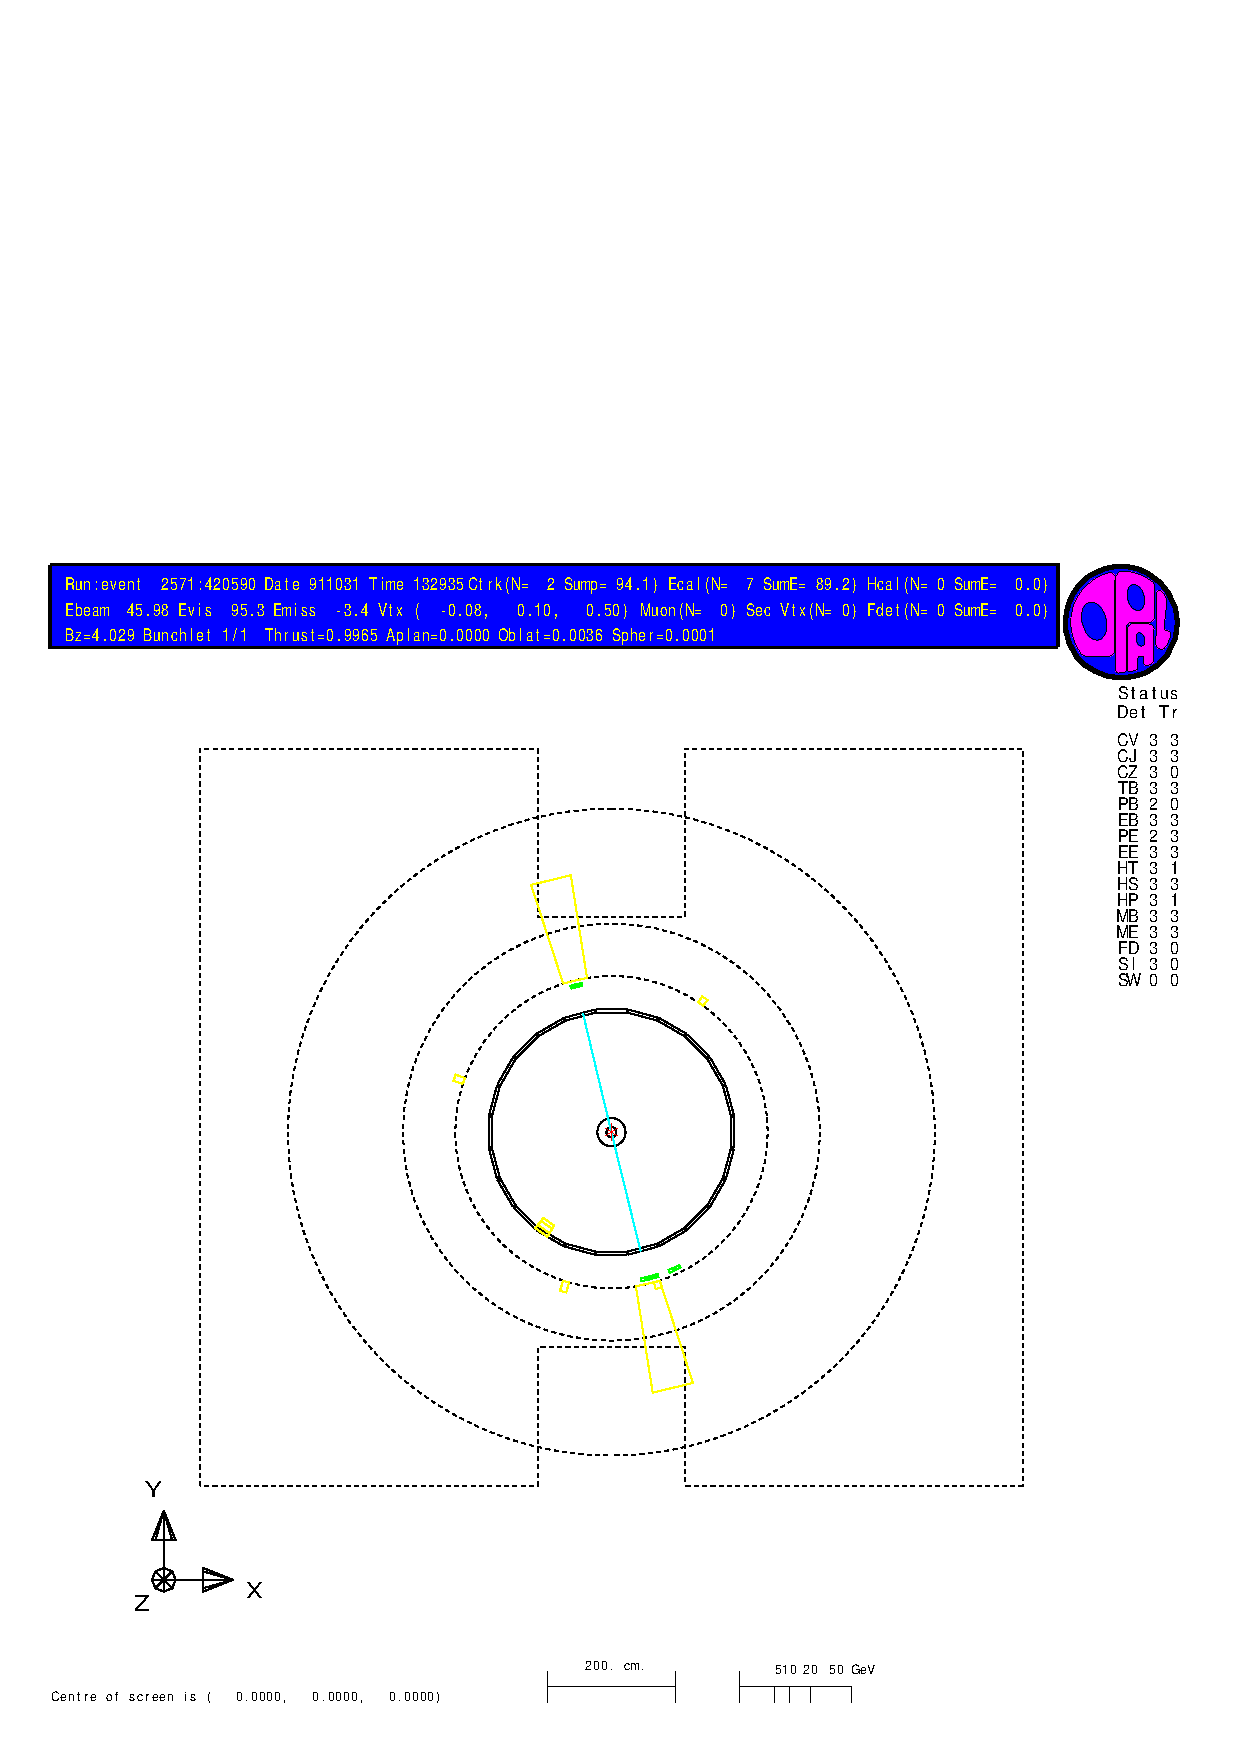
\includegraphics[width=\linewidth]{opal-electrons}
        \caption{%
            Electrons
        }
        \label{fig:grope/electrons}
    \end{subfigure}
    \hfill
    \begin{subfigure}[c]{0.48\linewidth}
        \centering
        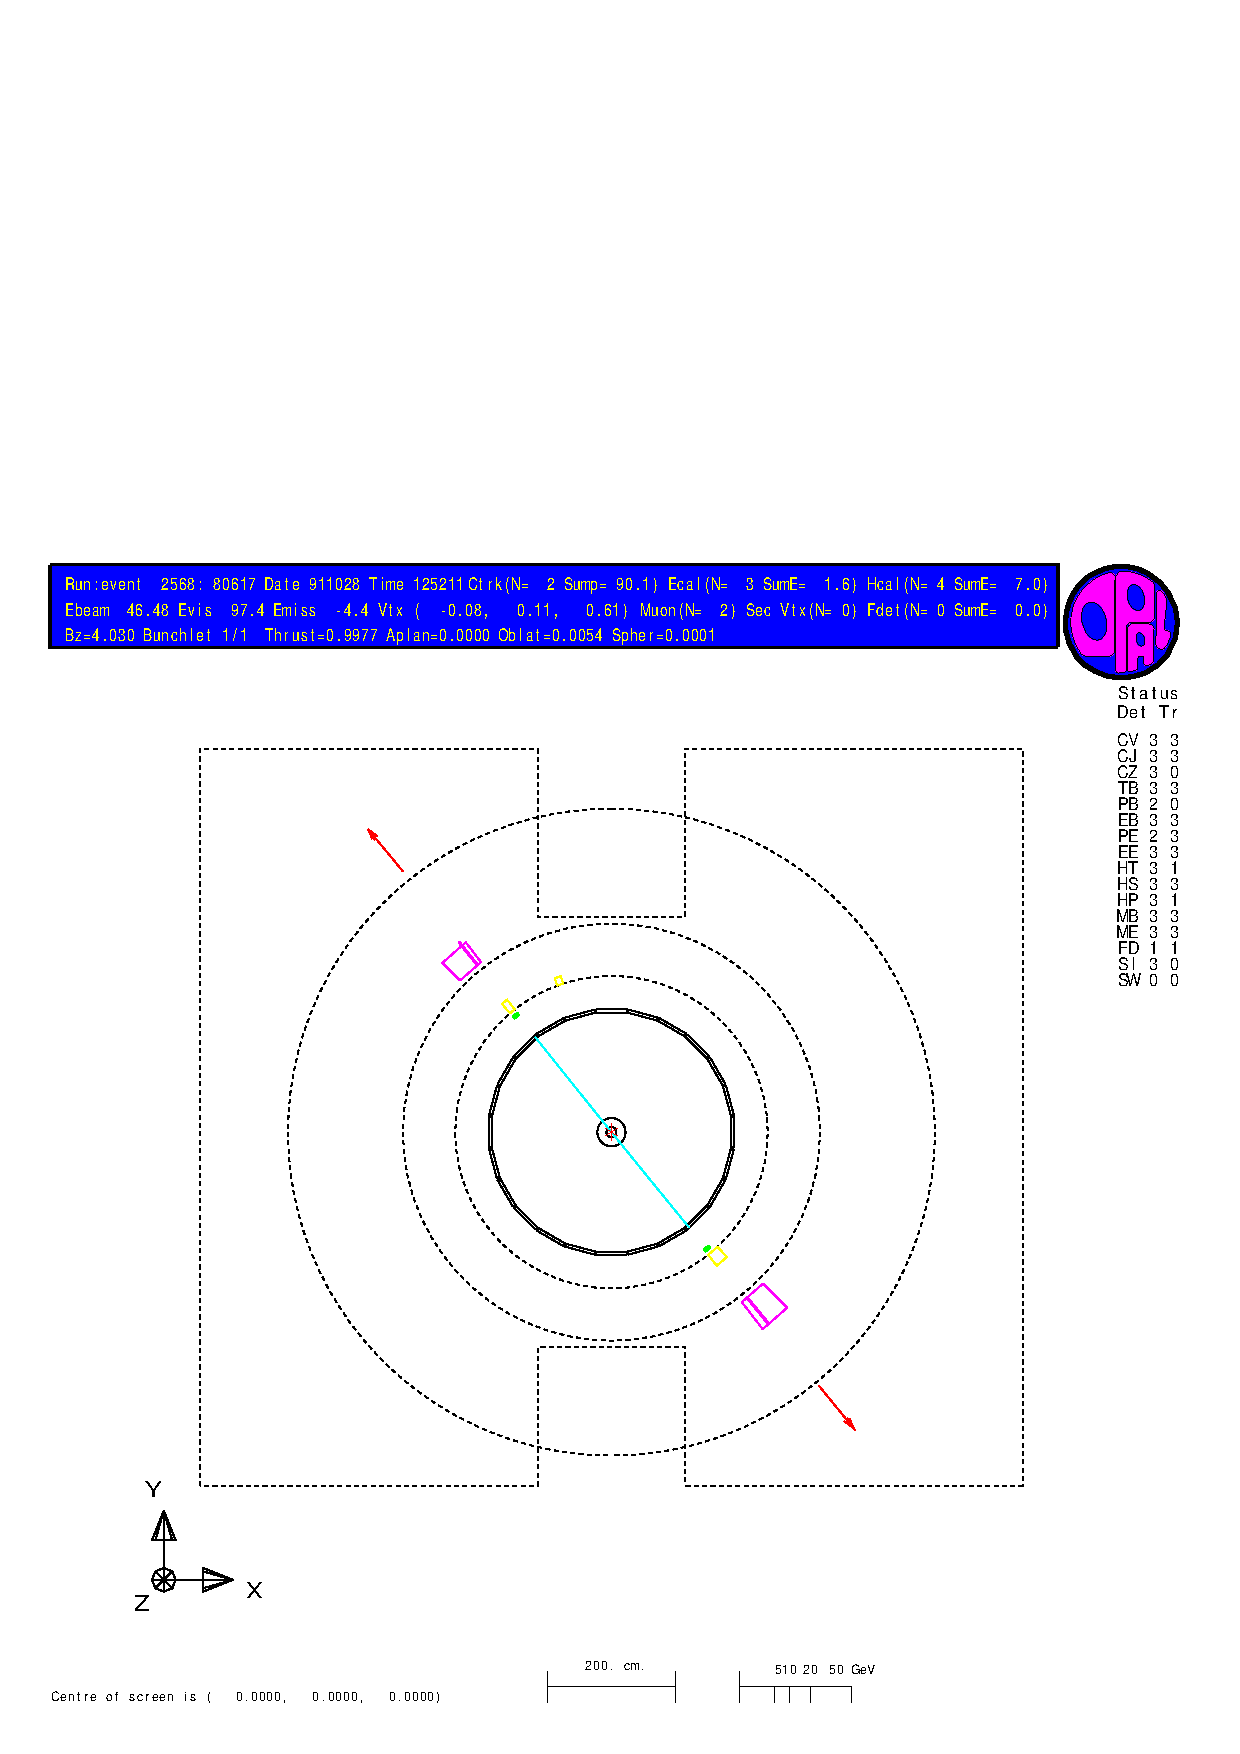
\includegraphics[width=\linewidth]{opal-muons}
        \caption{%
            Muons
        }
        \label{fig:grope/muons}
    \end{subfigure}

    \vspace{2ex}

    \begin{subfigure}[c]{0.48\linewidth}
        \centering
        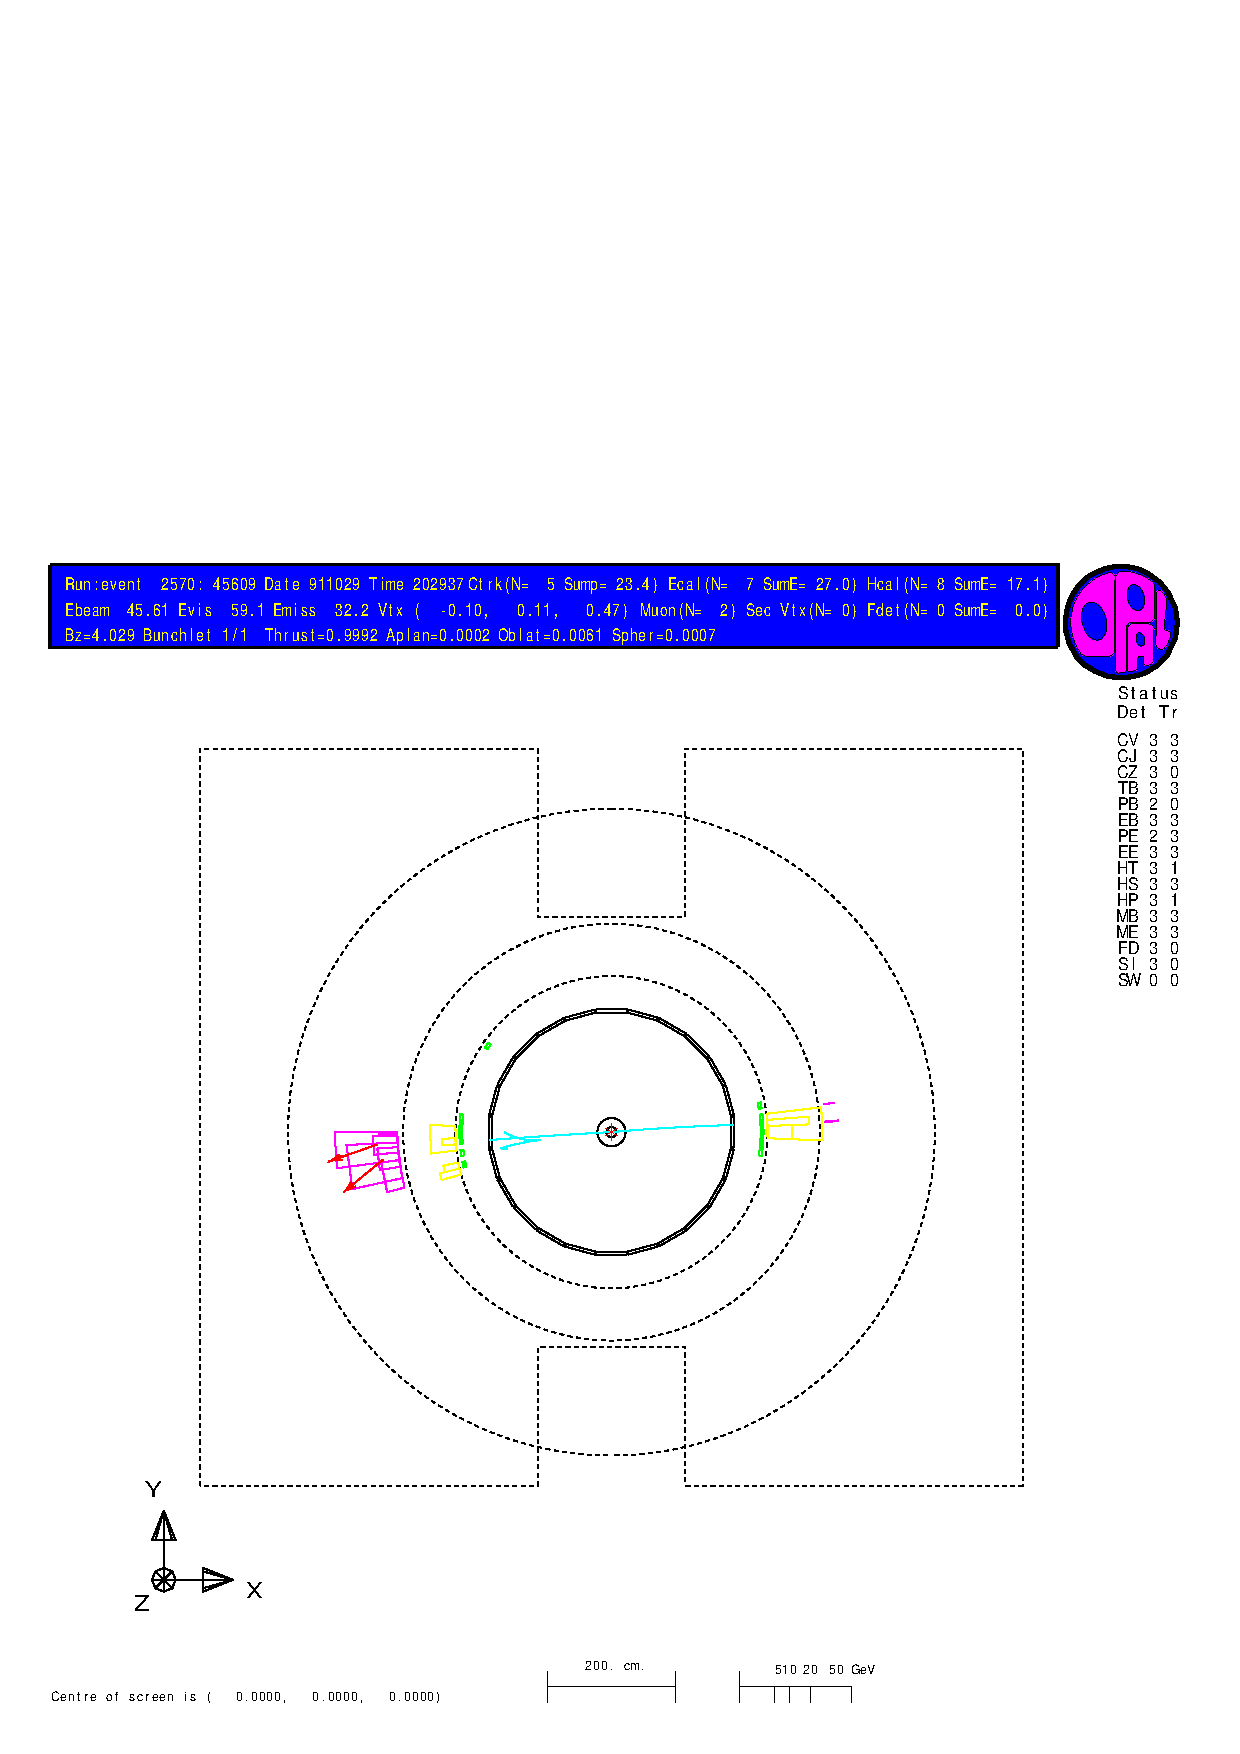
\includegraphics[width=\linewidth]{opal-taus}
        \caption{%
            Tauons
        }
        \label{fig:grope/tauons}
    \end{subfigure}
    \hfill
    \begin{subfigure}[c]{0.48\linewidth}
        \centering
        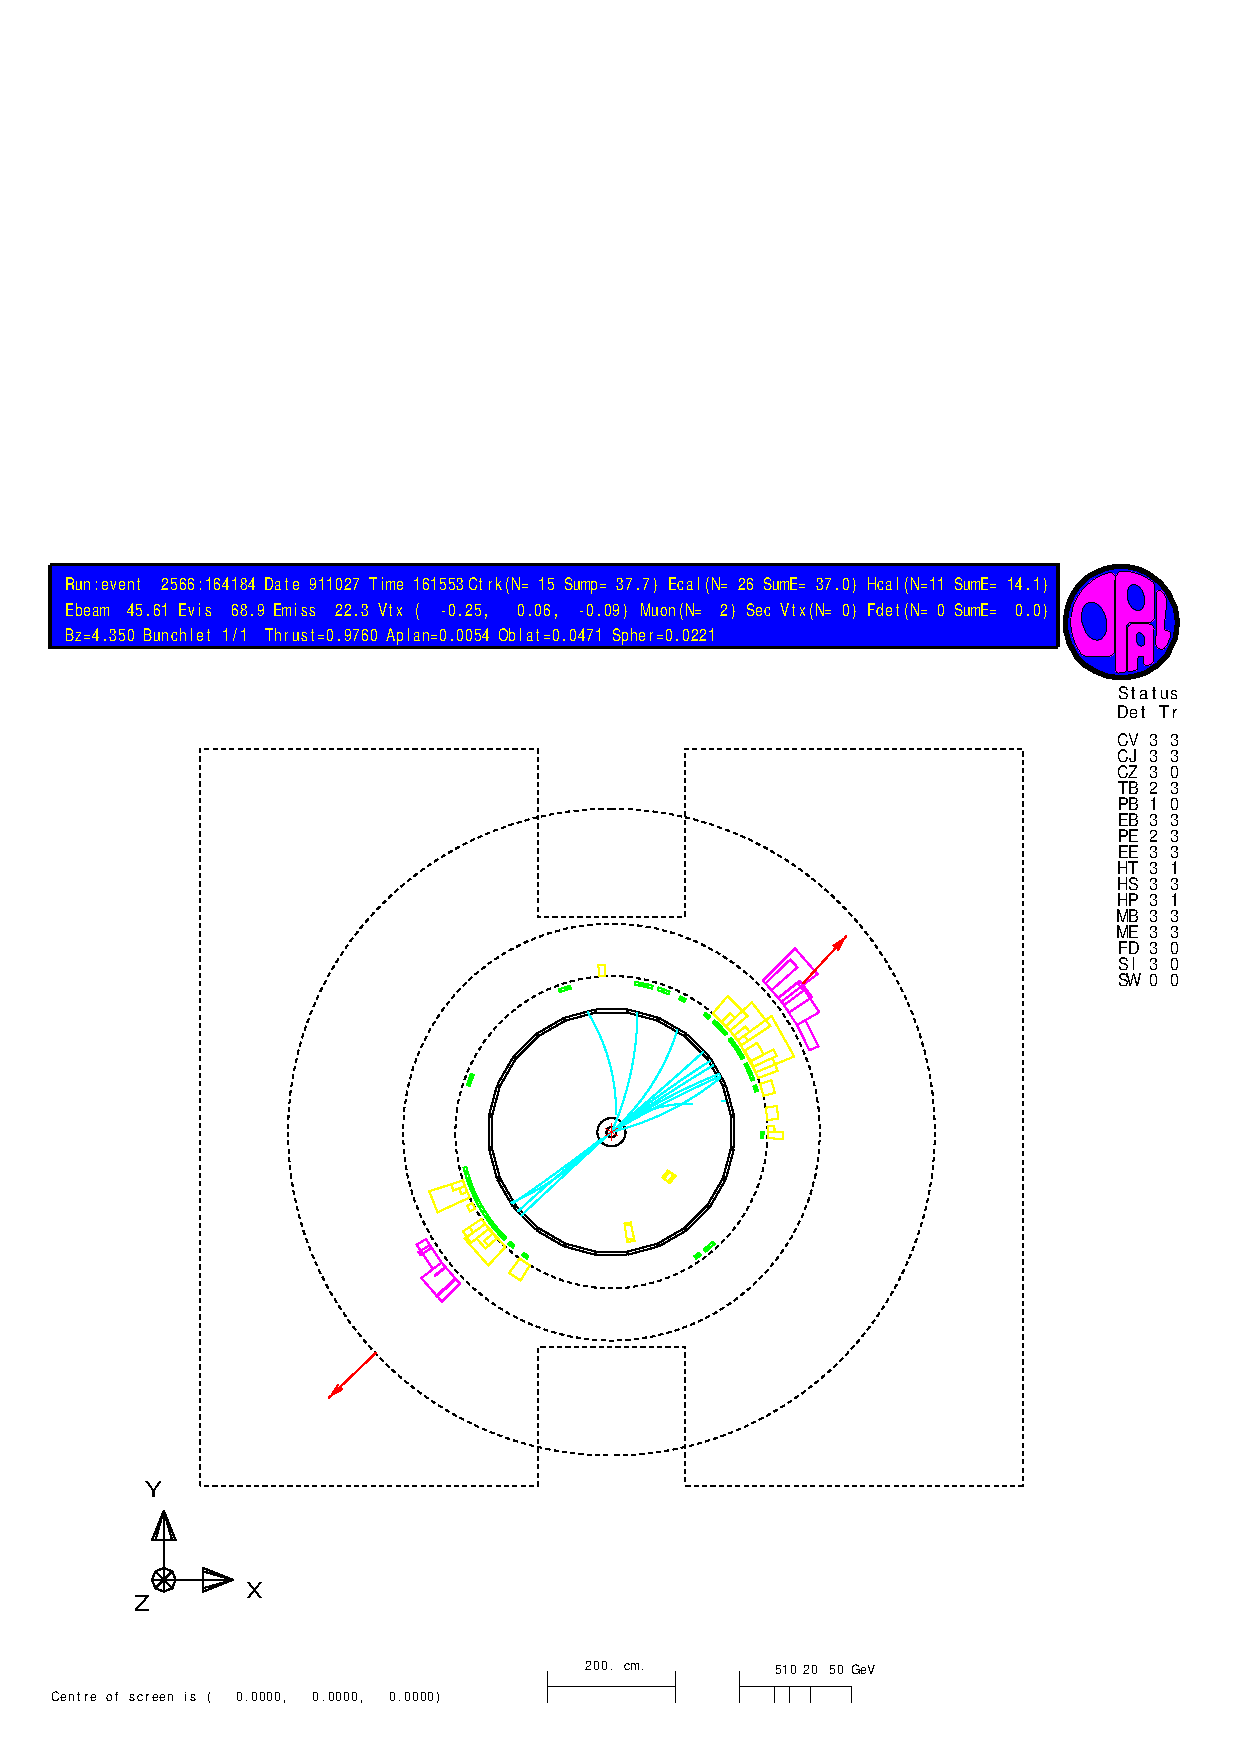
\includegraphics[width=\linewidth]{opal-hadrons}
        \caption{%
            Hadrons
        }
        \label{fig:grope/hadrons}
    \end{subfigure}
    \caption{%
        Event display of Monte Carlo events. One can see the traces from the
        vertex chamber in cyan, the hits in the \ecal{} are shown in yellow
        (probably hard to see on paper). In magenta, one has the hits in the
        \hcal{}. Muon penetrations are indicated with red arrows. Images are
        rendered with \textsc{grope}.
    }
    \label{fig:grope}
\end{figure}
